\section{LES ONDES ELECTROMAGNETIQUES}

%REFERENCE~: LIVRE PAGES 141 à 156

\subsection{Mise en situation}

\begin{figure}
\centering
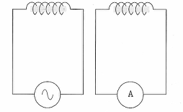
\includegraphics[width=7.297cm,height=4.45cm]{Pictures/10000001000000B7000000703138DA7480AE6A8A.png}
\caption{}
\end{figure}

Soit un premier circuit constitué d'une bobine soumise à une différence
de potentiel variable (courant alternatif).

Une seconde bobine, placée à quelques centimètres de la première n'est
pas raccordée à une source de courant mais est raccordée à un
ampèremètre (appareil qui mesure l'intensité du courant qui traverse le
circuit).

Nous observons que l'ampèremètre mesure un courant alternatif de même
fréquence que la fréquence du courant alternatif du premier circuit.

\subsection{Interprétation}

\emph{Une énergie s'est donc propagée, à travers l'air, du
premier circuit vers le deuxième.} Cette énergie a permis aux électrons
libres du second circuit de se déplacer et donc de créer un courant,
alternatif lui aussi.

(Soit dit en passant, c'est ainsi que fonctionnent les ondes radio, Gsm, \ldots. Nous les appellerons les ondes électromagnétiques).

\emph{MAIS QUELLE EST DONC CETTE FORME D'ENERGIE~? }

\emph{Rappel~:}

\emph{Une charge électrique produit dans son environnement un champ
électrique. }

\emph{Un champ électrique est une région de l'espace au sein de laquelle
une charge témoin subit une force. }

Les électrons libres du premier circuit oscillent (il s'agit d'un
courant alternatif) et donc ils produisent un champ électrique variable
dans l'espace. Les électrons libres du second circuit sont donc soumis à
cette variation de champ électrique, ils subissent la force électrique
variable et entrent en oscillation.

\subsubsection{Rappel~:}

\emph{Un courant électrique produit dans son environnement un champ
magnétique.}

\emph{Une variation de champ magnétique à l'intérieur d'une bobine
induit un courant électrique variable. }

Les électrons libres du premier circuit oscillent (il s'agit d'un
courant alternatif) et donc ils produisent un champ magnétique variable
dans l'espace. La seconde bobine est donc le siège d'un courant induit
variable.

\subsection{Spéculations de Maxwell}

Lorsque des charges en mouvement oscillent, elles produisent donc à la
fois un champ électrique et un champ magnétique variables dans le temps.
Maxwell a appelé \emph{ONDE ELECTROMAGNETIQUE cette propagation d'une
énergie stockée sous forme électrique et magnétique et produite par des
charges électriques oscillantes. }

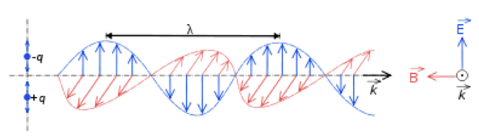
\includegraphics[width=15.993cm,height=4.634cm]{Pictures/10000001000001DF0000008BE924D8E1387D9253.png}

Les équations écrites par Maxwell (1865) montrent que le champ
électrique \[\overrightarrow{E}{}\] et le champ
magnétique\[\overrightarrow{B}{}\], engendrés par des charges
oscillantes (ici, un courant alternatif) ont les propriétés suivantes~:

\begin{itemize}
\item  Ils oscillent sinusoïdalement à la fréquence du courant.
\item  Ils transportent de l'énergie sous forme électrique et magnétique
  (électromagnétique donc).
\item  Ils sont perpendiculaires entre eux.
\end{itemize}

\emph{\textbf{Une onde électromagnétique est donc une forme d'énergie
qui se propage sous forme de «~paquet d'énergie~électromagnétique»,
produite par des charges oscillant à une certaine fréquence. Ce «~paquet
d'énergie~» est appelé un photon. }}

\subsection{Confirmation expérimentale}

En 1887, Hertz confirme expérimentalement les spéculations de Maxwell.
Utilisant des courants alternatifs de haute fréquence, il crée des ondes
électromagnétiques de longueur d'onde de l'ordre du mètre~: ce sont les
premières ondes hertziennes.

Poursuivant l'œuvre de Hertz, des physiciens (Marconi, Popov, Branly,
\ldots) contribuèrent à la mise au point d'un télégraphe sans fil. Cette
technique deviendra la base de la radiodiffusion et de ses prolongements
célèbres que sont la télévision et la mobilophonie.

Par la suite, on a montré que ces ondes peuvent être réfléchies,
réfractées, diffractées et qu'elles donnent lieu à des phénomènes
d'interférences. Elles ont un comportement ondulatoire, d'où leur nom
d'ondes électromagnétiques.

De plus, elles se déplacent toutes à la vitesse de la lumière.

\subsection{Gamme des ondes électromagnétiques}

La famille des ondes électromagnétiques peut être divisée en différentes
catégories~: chaque catégorie ayant son mode de production, de détection
et son domaine d'applications.

Chacune de ces catégories est caractérisée par une gamme de fréquence f
(et donc de longueur d'onde). Au plus la fréquence est grande, au plus
l'énergie de l'onde électromagnétique est grande.

Toutes les ondes électromagnétiques se déplacent à la vitesse de la
lumière au sein d'un milieu ou dans le vide.

\begin{figure}
\centering
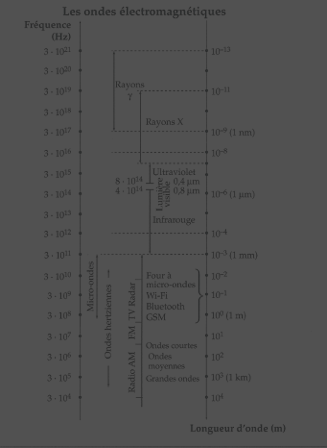
\includegraphics[width=11.425cm,height=14.616cm]{Pictures/1000000100000147000001C0C9C8D746CD882C9F.png}
\caption{}
\end{figure}

\begin{figure}
\centering
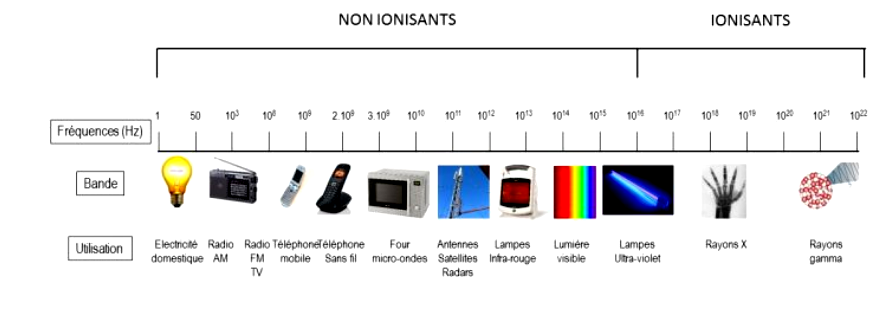
\includegraphics[width=17.233cm,height=6.184cm]{Pictures/100000010000037D0000014014F58CF6D7F0CE8B.png}
\caption{}
\end{figure}

En partant des ondes les plus
énergétiques (de plus grande fréquence), on distingue successivement : 
\begin{itemize}
\item
  \emph{\textbf{Les rayons gamma }}\textbf{(}γ\textbf{) :} ils sont dus
  aux radiations émises par les éléments radioactifs.\\
  Très énergétiques, ils traversent facilement la matière et sont très
  dangereux pour les cellules vivantes en cas d'excès.\\
\item \textbf{Les rayons X}  : rayonnements très énergétiques
  traversant plus ou moins facilement les corps matériels et un peu
  moins nocifs que les rayons gamma. Ils sont utilisés notamment en
  médecine pour les radiographies, dans l'industrie (contrôle des
  bagages dans le transport aérien) et dans la recherche pour l'étude de
  la matière (rayonnement synchrotron).\\
\item \textbf{Les ultraviolets} : rayonnements qui restent
  assez énergétiques. Heureusement pour nous, une grande part des
  ultraviolets émis par le soleil est stoppée par l'ozone atmosphérique
  qui sert de bouclier protecteur.
\item \textbf{Le domaine visible}: correspond à la partie
  très étroite du spectre électromagnétique perceptible par notre œil.
  Il s'agit de la lumière visible.\\
  \emph{Il s'étend de 400 nm (lumière bleue) à 800 nm (lumière rouge).}
\item  \textbf{L'infrarouge} : rayonnement émis par tous les
  corps dont la température est supérieure au zéro absolu (-273°C).\\
  En télédétection, on utilise certaines bandes spectrales de
  l'infrarouge pour mesurer la température des surfaces terrestres et
  océaniques, ainsi que celle des nuages.
\item \textbf{Les micro-ondes~}: 
  \begin{itemize}
  \item    \textbf{La télécommunication par satellite.}
  \item    \textbf{Les ondes radar~}: notamment utilisées en navigation
    maritime et aérienne. Dans la même gamme de fréquence, on trouve les
    ondes émises par les clés de verrouillage/déverrouillage automatique
    des portes de voiture.
  \item    \textbf{Dans les fours à micro-ondes} de cuisine, les molécules
    d'eau entrent en résonance et oscillent avec une grande amplitude.
    Cette énergie d'oscillation est rapidement transformée en énergie
    thermique par collisions avec les autres molécules.
  \item    \textbf{Wi-Fi} (Wireless Fidelity).
  \item    \textbf{Bluetooth}.
  \item
    La téléphonie mobile~: ondes \textbf{GSM} (Global System Mobile).
  \end{itemize}
\item \textbf{Les ondes hertziennes} : Ce domaine de
  longueurs d'onde concerne les ondes qui ont les plus basses
  fréquences. Il s'étend des longueurs d'onde de quelques cm à plusieurs
  km.
  \begin{itemize}
  \item    \textbf{Les ondes en télévision~}: transmission des images en
    télévision.
  \item    \textbf{Les ondes radio~}: relativement faciles à émettre et à
    recevoir, les ondes radio sont utilisées pour la transmission de
    l'information (radio).
  \end{itemize}
\end{itemize}

Nous sommes entourés d'ondes électromagnétiques au niveau domestique~: une petite illustration.

\begin{figure}
\centering
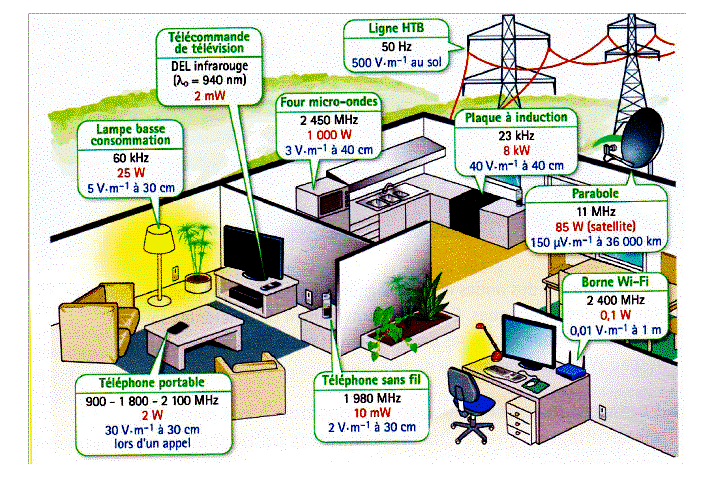
\includegraphics[width=15.847cm,height=10.767cm]{Pictures/10000001000002D5000001ED5EE60B9D153FD951.png}
\caption{}
\end{figure}
